\documentclass[aspectratio=169]{beamer}
% \documentclass{beamer}
\usepackage[utf8]{inputenc}
\usepackage{tikz}
\usepackage{booktabs}
\usepackage{hyperref}
\usepackage{amsmath}
\usepackage{amssymb}
\usepackage{xcolor}
\usepackage{colortbl}
\usepackage{graphicx}
\usepackage{tabularx}
\usepackage{array}
\usepackage{multicol}
\usepackage{ragged2e}

\usetikzlibrary{shapes,arrows,positioning,shadows,mindmap,trees,
                decorations.pathreplacing,calc,backgrounds,
                shapes.geometric,arrows.meta,fit,decorations.pathmorphing}

% ── EXACT COLOURS FROM PREAMBLE ──────────────────────────────
\definecolor{primary}{RGB}{0,102,204}
\definecolor{secondary}{RGB}{255,140,0}
\definecolor{accent}{RGB}{220,20,60}
\definecolor{success}{RGB}{40,167,69}
\definecolor{warning}{RGB}{255,193,7}
\definecolor{info}{RGB}{23,162,184}
\definecolor{light}{RGB}{248,249,250}
\definecolor{dark}{RGB}{52,58,64}
\definecolor{gradient1}{RGB}{74,144,226}
\definecolor{gradient2}{RGB}{143,67,238}
\definecolor{PrimaryBlue}{RGB}{0,114,188}
\definecolor{AccentOrange}{RGB}{237,125,49}
\definecolor{DeepGreen}{RGB}{0,176,80}
\definecolor{VibrantRed}{RGB}{192,0,0}
\definecolor{SubtleGray}{RGB}{242,242,242}
\definecolor{DarkText}{RGB}{64,64,64}

% ── HYPERLINK SETUP ───────────────────────────────────────────
\hypersetup{
  colorlinks=true,
  linkcolor=blue,
  urlcolor=secondary,
}

% ── BEAMER THEME ──────────────────────────────────────────────
\usetheme{Madrid}
\usecolortheme{default}
\setbeamercolor{block title}{bg=PrimaryBlue!80!white, fg=white}
\setbeamercolor{block body}{bg=SubtleGray}
\setbeamercolor{alertblock title}{bg=AccentOrange, fg=white}
\setbeamercolor{alertblock body}{bg=AccentOrange!10, fg=DarkText}
\setbeamercolor{block title example}{bg=DeepGreen,fg=white}
\setbeamercolor{block body example}{bg=DeepGreen!10,fg=DarkText}
\setbeamercolor{alerted text}{fg=VibrantRed}
\setbeamercolor{itemize item}{fg=PrimaryBlue}
\setbeamercolor{itemize subitem}{fg=AccentOrange}
\setbeamercolor{enumerate item}{fg=PrimaryBlue}
\setbeamercolor{section in toc}{fg=PrimaryBlue}

\setbeamerfont{frametitle}{size=\normalsize,series=\bfseries}
\setbeamerfont{block title}{size=\small,series=\bfseries}
\setbeamerfont{footline}{size=\tiny}
\setbeamertemplate{navigation symbols}{}
\setbeamertemplate{blocks}[rounded][shadow=true]
\setbeamertemplate{itemize items}[circle]
\setbeamertemplate{enumerate items}[circle]

% ── FOOTER ────────────────────────────────────────────────────
\title{JVM Monitoring and Profiling Framework}
\subtitle{Performance Monitoring, Debugging, and Runtime Analysis}
\author{Kattela Jwalin \and M N Risheendra \and Ankit Lama}
\date{\today}

% ── TIKZ SHORTHAND STYLES ─────────────────────────────────────
\tikzset{
  pbox/.style={draw=PrimaryBlue,fill=gradient1!20,rounded corners=5pt,
               minimum width=2.5cm,minimum height=0.65cm,
               font=\scriptsize\bfseries,text centered,line width=0.8pt},
  gbox/.style={draw=DeepGreen,fill=DeepGreen!15,rounded corners=5pt,
               minimum width=2.5cm,minimum height=0.65cm,
               font=\scriptsize\bfseries,text centered,line width=0.8pt},
  obox/.style={draw=AccentOrange,fill=AccentOrange!18,rounded corners=5pt,
               minimum width=2.5cm,minimum height=0.65cm,
               font=\scriptsize\bfseries,text centered,line width=0.8pt},
  rbox/.style={draw=VibrantRed,fill=VibrantRed!12,rounded corners=5pt,
               minimum width=2.5cm,minimum height=0.65cm,
               font=\scriptsize\bfseries,text centered,line width=0.8pt},
  dbox/.style={draw=PrimaryBlue,fill=warning!25,diamond,aspect=2.8,
               minimum width=2.6cm,minimum height=0.65cm,
               font=\tiny\bfseries,text centered,line width=0.8pt},
  arr/.style={-{Stealth[length=4.5pt,width=3.5pt]},PrimaryBlue,thick},
  arro/.style={-{Stealth[length=4pt,width=3pt]},AccentOrange,thick},
  arrg/.style={-{Stealth[length=4pt,width=3pt]},DeepGreen,thick},
}

\begin{document}

% ----------------------------------------------------------------
% SLIDE 1: Title Page
% ----------------------------------------------------------------
{
\usebackgroundtemplate{
  \includegraphics[width=\paperwidth,height=\paperheight]{Capture.PNG}
}
\begin{frame}[plain]
\end{frame}
}
% \begin{frame}[plain]
% \vspace{0.3cm}
% \begin{center}
% {\small \textbf{Aurora Higher Education and Research Academy}}\\
% {\small School of Engineering}\\[0.2cm]
% {\small \textbf{B.~Tech -- Sophomore Year -- CSE}}\\[0.1cm]
% {\small \textbf{Term -- II}}\\[0.4cm]
% {\Large \textbf{JVM Monitoring and Profiling Framework}}\\[0.3cm]
% {\normalsize Advanced Java Profiler and Debugger}\\[0.4cm]
% \begin{columns}[T]
% \begin{column}{0.5\textwidth}
% \small
% \textbf{Course Name:} Java Programming\\
% \textbf{Faculty:} Dr. Vemula Aruna\\
% \hspace*{1.2cm} Associate Professor\\
% \textbf{Course Code:} CSE
% \end{column}
% \begin{column}{0.5\textwidth}
% \small
% \textbf{LEARNING GROUP: 04}\\[0.2cm]
% \begin{tabular}{ll}
% \textbf{Student Names} & \textbf{Reg. No.}\\
% M N Risheendra & 241U1R1080\\
% Kattela Jwalin & 241U1R1088\\
% Ankit Lama & 241U1R1089\\
% \end{tabular}
% \end{column}
% \end{columns}
% \end{center}
% \end{frame}

% ── SLIDE 2 : OUTLINE ────────────────────────────────────────
\begin{frame}{Presentation Outline}
    \tableofcontents
\end{frame}

% ══════════════════════════════════════════════════════════════
%  SECTION 1 — ABSTRACT
% ══════════════════════════════════════════════════════════════
\section{Abstract}

\begin{frame}{Abstract}
  \begin{block}{Abstract}
    \small
    Modern Java applications are increasingly complex, making it hard to
    detect \textbf{performance bottlenecks}, \textbf{memory leaks}, and
    \textbf{runtime errors} manually.

    This project presents an \textbf{Advanced Java Profiler \& Debugger} —
    a tool that monitors Java applications in real time and delivers
    structured insights through a graphical interface.

    \begin{itemize}\itemsep2pt
      \item \textbf{Runtime Analysis:} tracks execution time and call frequency.
      \item \textbf{Call Graph:} shows relationships between methods.
      \item \textbf{Memory Analysis:} finds heap-heavy objects and leaks.
      \item \textbf{JShell Debugger:} test code without restarting apps.
    \end{itemize}

    Uses \textbf{Java Instrumentation API} and \textbf{JVMTI} to collect
    JVM data, displayed via \textbf{Java Swing} panels.
  \end{block}

  \begin{exampleblock}{Keywords}
    \small
    Java Profiling $\cdot$ Runtime Analysis $\cdot$ JVMTI $\cdot$
    Call Graph $\cdot$ Memory Analysis $\cdot$ Instrumentation $\cdot$
    Performance Monitoring $\cdot$ Debugging
  \end{exampleblock}
\end{frame}

% ══════════════════════════════════════════════════════════════
%  SECTION 2 — INTRODUCTION
% ══════════════════════════════════════════════════════════════
\section{Introduction}

\begin{frame}{Introduction: The Problem}
    \begin{alertblock}{Problem Statement}
        As Java programs scale, analyzing execution manually becomes nearly impossible. Developers face immense challenges in identifying performance issues, detecting logical errors, and understanding execution flow.
    \end{alertblock}
    
    \vspace{0.3cm}
    \textbf{The core issues include:}
    \begin{itemize}
        \item \textbf{Manual Complexity:} Large programs are extremely difficult to analyze by hand.
        \item \textbf{Hidden Bottlenecks:} Performance issues and memory leaks are hard to detect without specialized tools.
        \item \textbf{Debugging Time:} Tracing logical and runtime errors in complex applications is highly time-consuming.
        \item \textbf{Inaccessible Tooling:} Existing enterprise tools are often too complicated for beginners to grasp internally.
    \end{itemize}
\end{frame}

% ── SLIDE 4 : INTRO OVERVIEW ────────────────────────────────
\begin{frame}{Introduction: Overview}
  \begin{columns}[T]
    \column{0.54\textwidth}
      \textbf{Why do we need a Java Profiler?}
      \vspace{4pt}
      \begin{itemize}\itemsep4pt\small
        \item Java powers millions of \textbf{enterprise apps and web systems}.
        \item As code grows, \textbf{performance issues hide} inside the JVM.
        \item \textbf{Memory leaks} silently degrade application stability.
        \item \textbf{Slow methods} go unnoticed without precise measurement.
        \item Debugging \textbf{multi-threaded} code is notoriously error-prone.
        \item Existing tools are \textbf{complex for beginners} to use and understand.
      \end{itemize}

    \column{0.42\textwidth}
      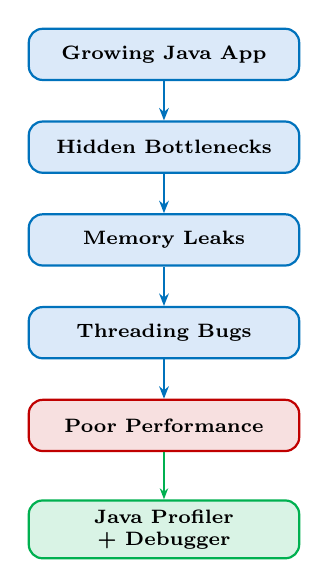
\begin{tikzpicture}[node distance=0.5cm]
        \node[pbox,text width=3.2cm] (a) {Growing Java App};
        \node[pbox,text width=3.2cm,below=of a] (b) {Hidden Bottlenecks};
        \node[pbox,text width=3.2cm,below=of b] (c) {Memory Leaks};
        \node[pbox,text width=3.2cm,below=of c] (d) {Threading Bugs};
        \node[rbox,text width=3.2cm,below=of d] (e) {Poor Performance};
        \node[gbox,text width=3.2cm,below=0.6cm of e] (f) {Java Profiler + Debugger};
        \draw[arr] (a)--(b); \draw[arr] (b)--(c);
        \draw[arr] (c)--(d); \draw[arr] (d)--(e);
        \draw[arrg] (e)--(f);
      \end{tikzpicture}
    \end{columns}
\end{frame}

% ── SLIDE 5 : OBJECTIVES ────────────────────────────────────
\begin{frame}{Introduction: Objectives}
The proposed system aims to:
\vspace{0.3cm}
\begin{enumerate}
  \item \textbf{Understand} the concept of program profiling and debugging in Java.
  \item \textbf{Analyze} the execution behaviour of Java applications at runtime.
  \item \textbf{Measure} performance metrics: execution time, call count, memory usage.
  \item \textbf{Identify} errors and inefficiencies in Java programs.
  \item \textbf{Develop} a simplified Java profiling and debugging system.
  \item \textbf{Visualize} method call graphs, memory maps, and execution snapshots.
  \item \textbf{Provide} an educational tool for understanding program execution.
  \item \textbf{Enhance} knowledge of software performance monitoring.
\end{enumerate}
\vspace{0.3cm}
\begin{exampleblock}{Core Philosophy}
\centering\small
\textbf{``Bridging JVM internals with developer-friendly performance insights.''}
\end{exampleblock}
\end{frame}

% ── SLIDE 6 : CONCEPTS — JVM + JAVA AGENT ───────────────────
\begin{frame}{Introduction: Key Concepts (Part I)}
\begin{columns}[T]

% ── LEFT SIDE ─────────────────────────────
\column{0.52\textwidth}

\begin{block}{JVM — Java Virtual Machine}
\small
The engine that \textbf{executes Java bytecode}. It manages memory,
threads, and garbage collection. All profiling happens inside the JVM.
\end{block}

\vspace{3pt}

\begin{block}{Java Agent}
\small
A plugin that \textbf{attaches before the application starts}.
It intercepts class loading and modifies bytecode without
changing source code.
\end{block}

\vspace{3pt}

\begin{block}{JVMTI — JVM Tool Interface}
\small
A \textbf{native C++ API} inside the JVM that provides low-level
access to threads, memory, method events, and GC callbacks.
\end{block}
% ── RIGHT SIDE ────────────────────────────
\column{0.48\textwidth}

\centering
      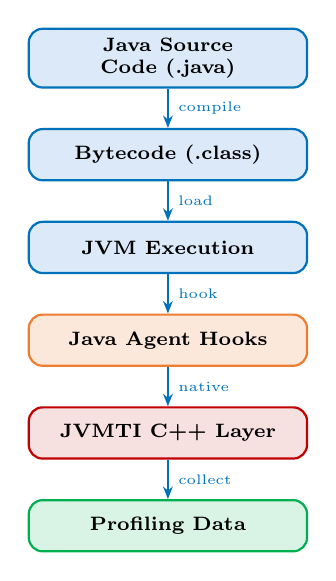
\begin{tikzpicture}[node distance=0.5cm]
        \node[pbox,text width=3.3cm] (src) {Java Source Code (.java)};
        \node[pbox,text width=3.3cm,below=of src] (bc) {Bytecode (.class)};
        \node[pbox,text width=3.3cm,below=of bc] (jvm) {JVM Execution};
        \node[obox,text width=3.3cm,below=of jvm] (agent) {Java Agent Hooks};
        \node[rbox,text width=3.3cm,below=of agent] (jvmti) {JVMTI C++ Layer};
        \node[gbox,text width=3.3cm,below=of jvmti] (data) {Profiling Data};
        \draw[arr] (src)--(bc) node[midway,right,font=\tiny]{compile};
        \draw[arr] (bc)--(jvm) node[midway,right,font=\tiny]{load};
        \draw[arr] (jvm)--(agent) node[midway,right,font=\tiny]{hook};
        \draw[arr] (agent)--(jvmti) node[midway,right,font=\tiny]{native};
        \draw[arr] (jvmti)--(data) node[midway,right,font=\tiny]{collect};
      \end{tikzpicture}
  \end{columns}
\end{frame}

% ── SLIDE 7 : CONCEPTS — INSTRUMENTATION + CALL GRAPH + MEMORY
\begin{frame}{Introduction: Key Concepts (Part II)}
  \begin{columns}[T, onlytextwidth]
    
    % ── LEFT SIDE ─────────────────────────────
    \column{0.52\textwidth}

    \begin{block}{Bytecode Instrumentation}
    \small
    Injecting \textbf{monitoring code into bytecode} at class-load time.
    The application runs normally while extra code records execution details.
    \end{block}
    
    \vspace{2pt}
    
    \begin{block}{Call Graph}
    \small
    A \textbf{directed graph} where nodes represent methods and edges show
    calling relationships. It helps identify execution flow and bottlenecks.
    \end{block}
    
    \vspace{2pt}
    
    \begin{block}{Memory Analysis}
    \small
    Tracks \textbf{heap allocation per class/object} using JVMTI callbacks.
    Helps identify high memory usage and detect leaks.
    \end{block}

    \column{0.45\textwidth}
      \vspace*{0.2cm}
      \begin{center}
        \scalebox{0.85}{
          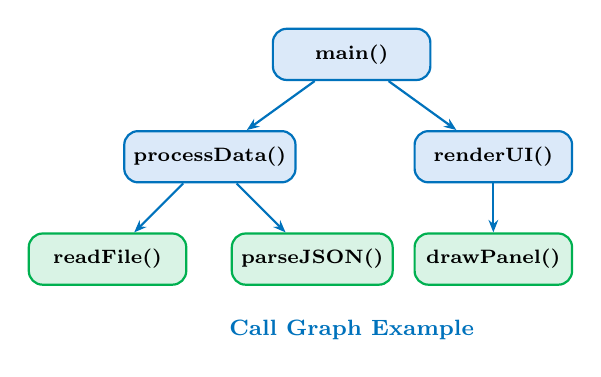
\begin{tikzpicture}
            % Perfectly symmetric relative layout to prevent overlaps
            \node[pbox, minimum width=2cm, font=\scriptsize\bfseries] (main) at (0, 0) {main()};
            
            \node[pbox, minimum width=2cm, font=\scriptsize\bfseries] (a) at (-1.8, -1.3) {processData()};
            \node[pbox, minimum width=2cm, font=\scriptsize\bfseries] (b) at (1.8, -1.3) {renderUI()};
            
            \node[gbox, minimum width=2cm, font=\scriptsize\bfseries] (c) at (-3.1, -2.6) {readFile()};
            \node[gbox, minimum width=2cm, font=\scriptsize\bfseries] (d) at (-0.5, -2.6) {parseJSON()};
            \node[gbox, minimum width=2cm, font=\scriptsize\bfseries] (e) at (1.8, -2.6) {drawPanel()};
            
            \draw[arr] (main) -- (a); 
            \draw[arr] (main) -- (b);
            \draw[arr] (a) -- (c); 
            \draw[arr] (a) -- (d);
            \draw[arr] (b) -- (e);
            
            \node[font=\footnotesize\bfseries\color{PrimaryBlue}] at (0, -3.5) {Call Graph Example};
          \end{tikzpicture}
        }
      \end{center}
  \end{columns}
\end{frame}

% ══════════════════════════════════════════════════════════════
%  SECTION 3 — LITERATURE SURVEY
% ══════════════════════════════════════════════════════════════
\section{Literature Survey}

% ── SLIDE 8 : LIT SURVEY PAPERS 1 & 2 ──────────────────────
\begin{frame}{Literature Survey: Research Review (Part I)}
  \footnotesize
  \begin{columns}[T]
    \column{0.48\textwidth}
      \begin{block}{\color{white}Burchell \& Marr — 2023}
        \textbf{Don't Trust Your Profiler: Precision \& Accuracy of Java Profilers}
        \begin{itemize}\scriptsize\itemsep3pt
          \item Evaluates multiple Java profilers — sampling vs instrumentation.
          \item \textbf{Key Finding:} Different tools produce \textbf{inconsistent} results
                for the same program.
          \item Instrumentation profilers add overhead; sampling misses short calls.
          \item \textbf{Gap:} No single tool gives reliably accurate data.
          \item Recommends combining both techniques for better accuracy.
        \end{itemize}
        \href{https://stefan-marr.de/downloads/mplr23-burchell-et-al-dont-trust-your-profiler.pdf}%
          {\textcolor{primary}{\textbf{[Access Paper]}}}
      \end{block}
    \column{0.48\textwidth}
      \begin{block}{\color{white}Burchell \& Marr — 2024}
        \textbf{Realistic Results for Instrumentation Profilers in JIT Systems}
        \begin{itemize}\scriptsize\itemsep3pt
          \item Investigates how bytecode instrumentation interferes with \textbf{JIT} compilation.
          \item Extra monitoring code disrupts JIT optimizations.
          \item \textbf{Gap:} Results don't reflect real-world application performance.
          \item Proposes \textbf{hybrid adaptive} profiling methods.
          \item Selective instrumentation only on critical sections reduces distortion.
        \end{itemize}
        \href{https://stefan-marr.de/downloads/mplr24-burchell-et-al-towards-realistic-results-for-instrumentation-based-profilers-for-jit-compiled-systems.pdf}%
          {\textcolor{primary}{\textbf{[Access Paper]}}}
      \end{block}
  \end{columns}
\end{frame}

% ── SLIDE 9 : LIT SURVEY PAPERS 3 & 4 ──────────────────────
\begin{frame}{Literature Survey: Research Review (Part II)}
  \footnotesize
  \begin{columns}[T]
    \column{0.48\textwidth}
      \begin{block}{\color{white}ASE Research Team — 2024}
        \textbf{Comparing CPU \& Memory Profiler Results Across Java Versions}
        \begin{itemize}\scriptsize\itemsep3pt
          \item Analyzes how profiling data \textbf{varies across different JVM versions}.
          \item JVM optimizations alter execution behaviour unpredictably.
          \item \textbf{Gap:} Profilers break when new JVM versions are released.
          \item Cross-version performance comparisons become unreliable.
          \item Recommends standardized, version-aware profiling frameworks.
        \end{itemize}
        \href{https://link.springer.com/article/10.1007/s10515-024-00423-2}%
          {\textcolor{primary}{\textbf{[Access Paper]}}}
      \end{block}
    \column{0.48\textwidth}
      \begin{block}{\color{white}Programming Journal — 2023}
        \textbf{Profiling and Optimizing Java Streams}
        \begin{itemize}\scriptsize\itemsep3pt
          \item Profiles Java \textbf{Stream API} operations to detect overhead.
          \item Parallel streams cause synchronization overhead in many cases.
          \item Complex pipelines reduce both readability and performance.
          \item \textbf{Gap:} Performance gains depend heavily on dataset size.
          \item Profiling reveals which stream operations to simplify or replace.
        \end{itemize}
        \href{https://programming-journal.org/2023/7/10/}%
          {\textcolor{primary}{\textbf{[Access Paper]}}}
      \end{block}
  \end{columns}
\end{frame}

% ── SLIDE 10 : LIT SURVEY TABLE I ───────────────────────────
\begin{frame}{Contemporary Research Innovations (Part I)}
\footnotesize
\renewcommand{\arraystretch}{1.2}
\begin{table}
\centering
\resizebox{0.95\textwidth}{!}{
\begin{tabular}{|>{\columncolor{gradient1!20}}p{2.8cm}|>{\columncolor{gradient2!20}}p{2.0cm}|>{\columncolor{success!20}}p{0.8cm}|>{\columncolor{warning!20}}p{4.3cm}|}
\hline
\rowcolor{primary!30}
\textbf{\color{white}Research Title} & \textbf{\color{white}Authors} & \textbf{\color{white}Year} & \textbf{\color{white}Innovation \& Impact} \\
\hline
\cellcolor{info!20}Don’t Trust Your Profiler: An Empirical Study & \cellcolor{secondary!20}T. Burchell, S. Marr & \cellcolor{accent!20}2023 & Evaluates profiler accuracy, comparing sampling vs. instrumentation. Shows that profiler outputs need careful interpretation. \href{https://stefan-marr.de/downloads/mplr23-burchell-et-al-dont-trust-your-profiler.pdf}{\textcolor{primary}{\textbf{[View PDF]}}} \\
\hline
\cellcolor{info!20}Towards Realistic Results for Instrumentation Profilers & \cellcolor{secondary!20}T. Burchell, S. Marr & \cellcolor{accent!20}2024 & Investigates how instrumentation disrupts JIT compilers. Suggests hybrid and adaptive methods for accurate environments. \href{https://stefan-marr.de/downloads/mplr24-burchell-et-al-towards-realistic-results-for-instrumentation-based-profilers-for-jit-compiled-systems.pdf}{\textcolor{primary}{\textbf{[View PDF]}}} \\
\hline
\cellcolor{info!20}Comparing CPU and Memory Profiler Results & \cellcolor{secondary!20}Automated SW Eng Team & \cellcolor{accent!20}2024 & Analyzes consistency across JVM versions. Proves JVM differences highly impact profiling data reliability. \href{https://link.springer.com/article/10.1007/s10515-024-00423-2}{\textcolor{primary}{\textbf{[View Link]}}} \\
\hline
\end{tabular}
}
\end{table}
\end{frame}

% --- SLIDE 11 ---
\begin{frame}{Contemporary Research Innovations (Part II)}
\footnotesize
\renewcommand{\arraystretch}{1.2}
\begin{table}
\centering
\resizebox{0.95\textwidth}{!}{
\begin{tabular}{|>{\columncolor{gradient1!20}}p{2.8cm}|>{\columncolor{gradient2!20}}p{2.0cm}|>{\columncolor{success!20}}p{0.8cm}|>{\columncolor{warning!20}}p{4.3cm}|}
\hline
\rowcolor{primary!30}
\textbf{\color{white}Research Title} & \textbf{\color{white}Authors} & \textbf{\color{white}Year} & \textbf{\color{white}Innovation \& Impact} \\
\hline
\cellcolor{info!20}Profiling and Optimizing Java Streams & \cellcolor{secondary!20}Programming Journal & \cellcolor{accent!20}2023 & Profiles Java Stream operations. Identifies inefficient stream operations to optimize performance while maintaining readability. \href{https://programming-journal.org/2023/7/10/}{\textcolor{primary}{\textbf{[View Link]}}} \\
\hline
\cellcolor{info!20}JVM Optimization: Empirical Analysis & \cellcolor{secondary!20}SoftwareX Research & \cellcolor{accent!20}2024 & Evaluates how JVM configurations (heap size, GC) affect web application performance and resource efficiency. \href{https://www.sciencedirect.com/science/article/pii/S2352711024003030}{\textcolor{primary}{\textbf{[View Link]}}} \\
\hline
\cellcolor{info!20}\textbf{JVM Profiler \& Debugger} & \cellcolor{secondary!20}\textbf{LG 04} & \cellcolor{accent!20}\textbf{2026} & \textbf{Integrates JVMTI + Java Agent + Swing UI for comprehensive real-time profiling with call graph and memory analysis.} \\
\hline
\end{tabular}
}
\end{table}
\end{frame}

% ══════════════════════════════════════════════════════════════
%  SECTION 5 — PROJECT DESIGN (IMAGE PLACEHOLDERS)
% ══════════════════════════════════════════════════════════════
\section{Project Design}

% ── SLIDE 17 : SYSTEM ARCHITECTURE (IMAGE) ──────────────────
\begin{frame}{Project Design: System Architecture}
  \begin{columns}[T]
    
    % ── LEFT SIDE (IMAGE) ─────────────────────────────
    \column{0.55\textwidth}
      \begin{figure}
        \centering
        \includegraphics[
          width=1.05\textwidth,
          height=0.65\textheight,
          keepaspectratio
        ]{architecture.png}
      \end{figure}
    
    % ── RIGHT SIDE (TEXT) ─────────────────────────────
    \column{0.42\textwidth}
      \small
      The architecture has \textbf{three layers}:
      
      \vspace{4pt}
      
      \begin{block}{Frontend}
        \texttt{ProfilerUI} — displays call graphs, memory maps, and execution snapshots.
      \end{block}
      
      \vspace{4pt}
      
      \begin{block}{Processing}
        \texttt{Profiler Engine} coordinates operations; \texttt{DataSender} transmits data.
      \end{block}
      
      \vspace{4pt}
      
      \begin{block}{JVM Layer}
        \texttt{Java Agent} + \texttt{JVMTI C++} agent hook into JVM to collect raw data.
      \end{block}

  \end{columns}
\end{frame}

% ── SLIDE 18 : USE CASE DIAGRAM (IMAGE) ─────────────────────
\begin{frame}{Project Design: Use Case Diagram}
  \begin{columns}[T]
    
    % ── LEFT SIDE (IMAGE) ─────────────────────────────
    \column{0.6\textwidth}
      \begin{figure}
        \centering
        \includegraphics[
          width=1.4\textwidth,
          height=0.82\textheight,
          keepaspectratio
        ]{usecase.png}
      \end{figure}
      
    \column{0.42\textwidth}
      \small
      \textbf{Actor: User / Developer}
      \vspace{4pt}
      \begin{itemize}\itemsep4pt\scriptsize
        \item \textbf{Load Program} — upload target Java application.
        \item \textbf{Profile Session} — start monitoring CPU, memory, method calls.
        \item \textbf{View Call Graph} — visualize method relationships.
        \item \textbf{Analyze Memory} — inspect heap usage per class.
        \item \textbf{Use JShell} — run interactive code snippets.
        \item \textbf{View Analytics} — graphs, timelines, and snapshots.
      \end{itemize}
  \end{columns}
\end{frame}

% ── SLIDE 21 : WORKING STEPS DIAGRAM (IMAGE) ────────────────
{
\usebackgroundtemplate{
  \includegraphics[width=\paperwidth,height=\paperheight]{workflow.png}
}
\begin{frame}[plain]{Project Design: System Workflow}
\end{frame}
}

% ══════════════════════════════════════════════════════════════
%  SECTION 4 — METHODOLOGY
% ══════════════════════════════════════════════════════════════
\section{Methodology}

% ── SLIDE 12 : METHODOLOGY OVERVIEW ─────────────────────────
\begin{frame}{Methodology: Overview}
  \begin{columns}[T]
    \column{0.52\textwidth}
      \small
      The system follows a \textbf{structured 8-step pipeline} from
      program execution to real-time visualization.
      \vspace{6pt}
      \begin{enumerate}\itemsep3pt\scriptsize
        \item \textbf{Application Launch} — app starts with agent attached via \texttt{-javaagent}.
        \item \textbf{Agent Initialization} — JVMTI hooks for method entry/exit enabled.
        \item \textbf{Method Interception} — every method call captured with timestamp.
        \item \textbf{Data Collection} — stored in \texttt{ProfilerRegistry} and \texttt{MethodStats}.
        \item \textbf{Native Layer} — C++ JVMTI agent collects memory and thread data.
        \item \textbf{Data Transmission} — \texttt{DataSender} sends data via socket.
        \item \textbf{Visualization} — \texttt{ProfilerUI} renders call graph, memory map, snapshots.
        \item \textbf{User Interaction} — load, analyze, and explore results.
      \end{enumerate}
    \column{0.44\textwidth}
      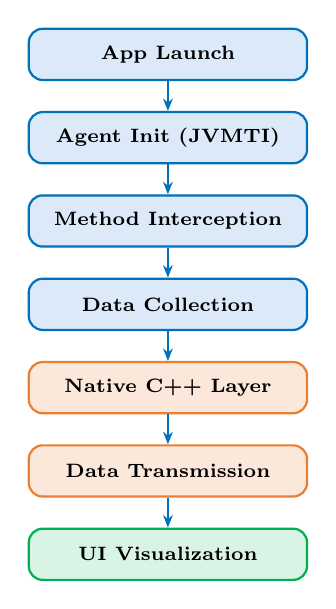
\begin{tikzpicture}[node distance=0.38cm]
        \node[pbox,text width=3.3cm] (a) {App Launch};
        \node[pbox,text width=3.3cm,below=of a] (b) {Agent Init (JVMTI)};
        \node[pbox,text width=3.3cm,below=of b] (c) {Method Interception};
        \node[pbox,text width=3.3cm,below=of c] (d) {Data Collection};
        \node[obox,text width=3.3cm,below=of d] (e) {Native C++ Layer};
        \node[obox,text width=3.3cm,below=of e] (f) {Data Transmission};
        \node[gbox,text width=3.3cm,below=of f] (g) {UI Visualization};
        \draw[arr] (a)--(b); \draw[arr] (b)--(c); \draw[arr] (c)--(d);
        \draw[arr] (d)--(e); \draw[arr] (e)--(f); \draw[arr] (f)--(g);
      \end{tikzpicture}
  \end{columns}
\end{frame}

% ── SLIDE 13 : THEORETICAL FOUNDATION ───────────────────────
\begin{frame}{Methodology: Theoretical Foundation}
    \begin{columns}
        \begin{column}{0.6\textwidth}
            \textbf{Bytecode Modification Theory}
            \begin{itemize}
                \item At load time, the \texttt{ClassFileTransformer} intercepts raw bytes.
                \item Logical \textit{Hooks} are injected at entry/exit points of designated methods.
            \end{itemize}
            \vspace{0.3cm}
            \textbf{Data Aggregation Logic}
            \begin{itemize}
                \item Continuous data stream is processed using concurrent hash-based structures to ensure thread safety without halting the JVM.
            \end{itemize}
        \end{column}
        \begin{column}{0.35\textwidth}
            \centering
            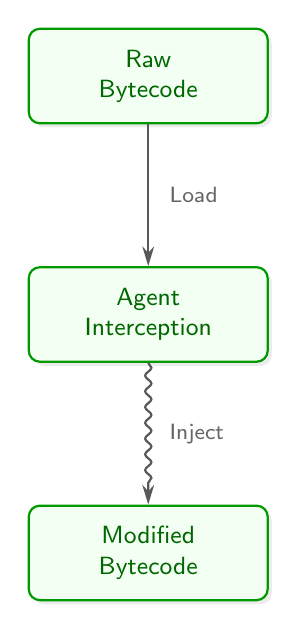
\begin{tikzpicture}[
    node distance=1.8cm,
    block/.style={
      rectangle, 
      rounded corners=4pt,
      draw=green!60!black, 
      fill=green!05, 
      text=green!40!black,
      thick, 
      minimum height=1.2cm, 
      text width=2.8cm, 
      align=center,
      font=\sffamily\small,
      drop shadow={opacity=0.15, shadow xshift=1.5pt, shadow yshift=-1.5pt}
    },
    arrow/.style={
      -{Stealth[length=2.5mm, width=1.5mm]}, 
      thick, 
      draw=gray!70!black
    },
    snake arrow/.style={
      arrow,
      decorate, 
      decoration={snake, amplitude=0.4mm, segment length=2mm, post length=2.5mm}
    },
    label/.style={
      right,
      font=\sffamily\footnotesize,
      text=gray!80!black,
      xshift=4pt % Gives the text some breathing room from the arrow
    }
  ]
    
    \node[block] (b1) {Raw\\Bytecode};
    \node[block, below=of b1] (b2) {Agent\\Interception};
    \node[block, below=of b2] (b3) {Modified\\Bytecode};
    
    \draw[arrow] (b1) -- node[label] {Load} (b2);
    \draw[snake arrow] (b2) -- node[label] {Inject} (b3);
    
  \end{tikzpicture}
        \end{column}
    \end{columns}
\end{frame}

% ── SLIDE 14 : ALGORITHMS — PART I ──────────────────────────
\begin{frame}{Methodology: Algorithms Used (Part I)}
  \begin{columns}[T]
    
    % ── LEFT SIDE ─────────────────────────────
    \column{0.50\textwidth}
      \begin{block}{1. Method Execution Tracking}
\begin{itemize}\scriptsize\itemsep3pt
  \item Hook fires on \textbf{method entry} and \textbf{method exit}.
  \item Capture \texttt{System.nanoTime()} at both points.
  \item \textbf{Execution Time} $= T_{exit} - T_{entry}$
  \item \textbf{Call Count} incremented on every entry event.
  \item Data stored per method in \texttt{MethodStats} object.
\end{itemize}
\end{block}

\vspace{6pt}

\begin{block}{2. Call Graph Construction}
\begin{itemize}\scriptsize\itemsep3pt
  \item Maintains a \textbf{thread-local call stack}.
  \item On entry: push current method; record caller $\to$ callee edge.
  \item On exit: pop method from stack.
  \item Builds a \textbf{directed graph}: Nodes = Methods, Edges = Calls.
  \item Graph rendered visually in \texttt{CallGraphPanel}.
\end{itemize}
\end{block}
      
    % ── RIGHT SIDE (TIKZ) ─────────────────────────────
    \column{0.46\textwidth}
      \centering
      \vspace{2pt}
      
      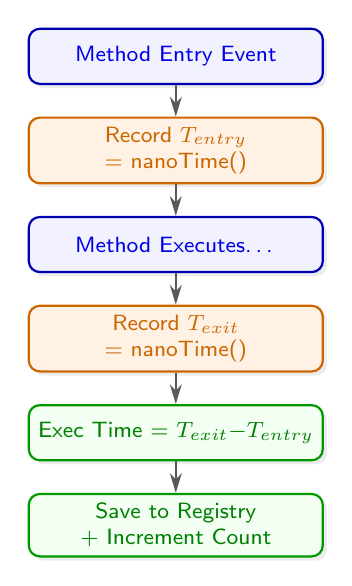
\begin{tikzpicture}[
    node distance=0.4cm, % Controls the exact length of the arrows
    basebox/.style={
      rectangle,
      rounded corners=4pt,
      thick,
      align=center,
      text width=3.5cm,
      minimum height=0.7cm,
      font=\sffamily\footnotesize, % Much cleaner and more readable than \tiny\bfseries
      drop shadow={opacity=0.15, shadow xshift=1.5pt, shadow yshift=-1.5pt}
    },
    pbox/.style={basebox, draw=blue!70!black, fill=blue!05, text=blue!90!black},
    obox/.style={basebox, draw=orange!80!black, fill=orange!10, text=orange!80!black},
    gbox/.style={basebox, draw=green!60!black, fill=green!05, text=green!50!black},
    arr/.style={-{Stealth[length=2.5mm, width=1.5mm]}, thick, draw=gray!70!black}
  ]

    % Nodes
    \node[pbox] (entry) {Method Entry Event};
    \node[obox, below=of entry] (t1) {Record $T_{entry}$ = nanoTime()};
    \node[pbox, below=of t1] (exec) {Method Executes\dots};
    \node[obox, below=of exec] (t2) {Record $T_{exit}$ = nanoTime()};
    \node[gbox, below=of t2] (calc) {Exec Time = $T_{exit}-T_{entry}$};
    
    % Split the last node into two lines for better visual balance inside the 3.5cm width
    \node[gbox, below=of calc] (save) {Save to Registry \\ + Increment Count};

    % Arrows
    \draw[arr] (entry) -- (t1); 
    \draw[arr] (t1) -- (exec);
    \draw[arr] (exec) -- (t2); 
    \draw[arr] (t2) -- (calc);
    \draw[arr] (calc) -- (save);
    
  \end{tikzpicture}
      
  \end{columns}
\end{frame}

% ── SLIDE 15 : ALGORITHMS — PART II ─────────────────────────
\begin{frame}{Methodology: Algorithms Used (Part II)}
  \begin{columns}[T]
    \column{0.48\textwidth}
      \begin{block}{3. Aggregation Algorithm}
        \begin{itemize}\scriptsize\itemsep3pt
          \item Uses \textbf{ConcurrentHashMap} for thread-safe storage.
          \item Key: method signature; Value: \texttt{MethodStats} object.
          \item Stores \textbf{cumulative} total time and total call count.
          \item Dynamically updates on every intercepted call.
          \item Enables real-time statistics without locking the app.
        \end{itemize}
      \end{block}
      \vspace{1pt}
      \begin{block}{4. Memory Tracking (JVMTI)}
        \begin{itemize}\scriptsize\itemsep3pt
          \item JVMTI registers \textbf{VMObjectAlloc callback}.
          \item Fires every time any object is allocated on heap.
          \item Tracks \textbf{memory usage per class/module}.
          \item Data shown in \texttt{MemoryMapPanel} as live chart.
        \end{itemize}
      \end{block}
    \column{0.48\textwidth}
      \begin{block}{5. Thread Monitoring}
        \begin{itemize}\scriptsize\itemsep3pt
          \item JVMTI captures \textbf{ThreadStart} and \textbf{ThreadEnd} events.
          \item Associates each method call with its \textbf{Thread ID}.
          \item Tracks number of active threads and their execution patterns.
          \item Helps detect \textbf{thread contention} and deadlocks.
        \end{itemize}
      \end{block}
      \vspace{6pt}
      \begin{exampleblock}{Performance Metrics Collected}
        \scriptsize
        \begin{tabular}{@{}ll@{}}
          \textbf{Exec Time} & $T_{exit} - T_{entry}$ \\
          \textbf{Call Count} & Counter per method \\
          \textbf{Heap Usage} & Per class (bytes) \\
          \textbf{Call Depth} & Graph traversal depth \\
          \textbf{Thread Count} & Active threads at runtime \\
          \textbf{CPU (indirect)} & Freq $\times$ Duration \\
        \end{tabular}
      \end{exampleblock}
  \end{columns}
\end{frame}

% ── SLIDE 16 : SYSTEM FLOWCHART ─────────────────────────────
\begin{frame}[plain]{Methodology: System Flowchart}
\centering
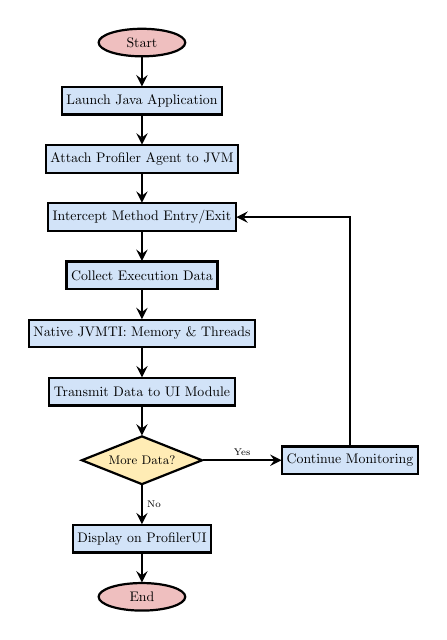
\begin{tikzpicture}[
  scale=0.5, transform shape,
  node distance=0.75cm,
  >=stealth,
  start/.style={ellipse, draw, fill=VibrantRed!25, minimum width=2.2cm, minimum height=0.7cm, align=center, font=\normalsize, thick},
  proc/.style={rectangle, draw, fill=gradient1!25, minimum width=3.2cm, minimum height=0.7cm, align=center, font=\normalsize, thick},
  dec/.style={diamond, draw, fill=warning!30, aspect=2.5, align=center, font=\small, thick},
  arr/.style={->, thick}
]
\node[start] (start) {Start};
\node[proc, below=of start] (launch) {Launch Java Application};
\node[proc, below=of launch] (attach) {Attach Profiler Agent to JVM};
\node[proc, below=of attach] (intercept) {Intercept Method Entry/Exit};
\node[proc, below=of intercept] (collect) {Collect Execution Data};
\node[proc, below=of collect] (native) {Native JVMTI: Memory \& Threads};
\node[proc, below=of native] (send) {Transmit Data to UI Module};
\node[dec, below=of send] (more) {More Data?};
\node[proc, right=2.0cm of more] (loop) {Continue Monitoring};
\node[proc, below=1.0cm of more] (display) {Display on ProfilerUI};
\node[start, below=of display] (end) {End};

\draw[arr] (start)--(launch);
\draw[arr] (launch)--(attach);
\draw[arr] (attach)--(intercept);
\draw[arr] (intercept)--(collect);
\draw[arr] (collect)--(native);
\draw[arr] (native)--(send);
\draw[arr] (send)--(more);
\draw[arr] (more.east)--node[above]{\scriptsize Yes}(loop);
\draw[arr] (loop)|-(intercept);
\draw[arr] (more.south)--node[right]{\scriptsize No}(display);
\draw[arr] (display)--(end);
\end{tikzpicture}
\end{frame}

% ══════════════════════════════════════════════════════════════
%  SECTION 6 — IMPLEMENTATION
% ══════════════════════════════════════════════════════════════
\section{Implementation}

% --- SLIDE 1: Core Implementation - Initialization & Interception ---
\begin{frame}{Core Implementation: Initialization \& Interception}
    \begin{block}{Step 1: Agent Initialization (\texttt{ProfilerAgent.java})}
        \small
        The agent uses the \texttt{premain()} method to attach to the JVM before the main app starts. It registers a \texttt{ClassFileTransformer} to enable runtime bytecode modification seamlessly without altering the original source code.
    \end{block}

    \vspace{0.3cm}

    \begin{block}{Step 2: Method Interception (\texttt{MethodInterceptor.java})}
        \small
        Target methods are dynamically wrapped to capture precise execution metrics. The flow follows:
        \begin{itemize}
            \item \textbf{Pre-execution:} Captures the start time just before execution begins.
            \item \textbf{Execution:} Invokes the original method logic.
            \item \textbf{Post-execution:} Captures the end time safely within a \texttt{finally} block.
            \item \textbf{Dispatch:} Calculates the duration and dispatches it to the central registry.
        \end{itemize}
    \end{block}
\end{frame}
% --- SLIDE 2: Core Implementation - Data Handling & Transmission ---
\begin{frame}{Core Implementation: Data Handling \& Transmission}
    \begin{columns}[T]
        % Left Column: Storage and Calculation
        \begin{column}{0.48\textwidth}
            \begin{exampleblock}{Step 3: Data Collection}
                \small \textbf{\texttt{ProfilerRegistry.java}}\\
                All intercepted data flows here. It utilizes a \texttt{ConcurrentHashMap<String, MethodStats>} to ensure that data inserted concurrently by multiple application threads does not cause race conditions.
            \end{exampleblock}
            
            \begin{exampleblock}{Step 4: Statistics Calculation}
                \small \textbf{\texttt{MethodStats.java}}\\
                Each individual method profile is tracked as an object. It actively increments \texttt{callCount} and compounds \texttt{totalTime}, forming the mathematical basis for the UI.
            \end{exampleblock}
        \end{column}

        % Right Column: Networking
        \begin{column}{0.48\textwidth}
            \begin{alertblock}{Step 5: Data Transmission}
                \small \textbf{\texttt{DataSender.java}}\\
                Since the monitored application and the visualizer may run independently, custom socket communication (via \texttt{localhost:9998}) is established. 
                
                \vspace{0.2cm}
                This module serializes and transmits the \texttt{ProfilerRegistry} statistics to the UI listener continuously in real-time, ensuring the dashboard is always up to date.
            \end{alertblock}
        \end{column}
    \end{columns}
\end{frame}

% --- SLIDE 3: Core Implementation - Native Layer & Visualization ---
\begin{frame}{Core Implementation: Native Layer \& Visualization}
    \begin{alertblock}{Step 6: JVMTI Native Integration (\texttt{agent.cpp})}
        \small
        A native C++ agent is loaded alongside the Java agent using the \texttt{Agent\_OnLoad} hook. This bypasses standard Java limits, performing deep heap scans to extract raw instance data and byte sizes directly from the JVM.
    \end{alertblock}

    \begin{columns}[T]
        % Left Column: UI Bootup
        \begin{column}{0.48\textwidth}
            \begin{block}{Step 7: UI Initialization}
                \small \textbf{\texttt{Launcher.java}}\\
                Acts as the entry point for the visualizer. It boots up the Java Swing framework, preparing the canvas and active listeners for incoming socket data.
            \end{block}
        \end{column}
        
        % Right Column: UI Rendering
        \begin{column}{0.48\textwidth}
            \begin{block}{Step 8: Displaying Profiling Data}
                \small \textbf{\texttt{ProfilerUI.java}}\\
                Features an \texttt{updateData()} routine that unpacks the serialized maps and triggers repaints on:
                \begin{itemize}
                    \item \textbf{Call Graphs}
                    \item \textbf{Execution Time Tables}
                    \item \textbf{Memory Usage Bar Charts}
                \end{itemize}
            \end{block}
        \end{column}
    \end{columns}
\end{frame}

% ── SLIDE 24 : TECHNOLOGIES USED ────────────────────────────
% ── SLIDE 1 ─────────────────────────────
\begin{frame}{Implementation: Technologies Used (Part I)}
  \begin{columns}[T]
    
    \column{0.48\textwidth}
      \begin{block}{Programming Languages}
        \begin{itemize}\normalsize\itemsep5pt
          \item \textbf{Java} — Core agent, UI, registry, data transfer.
          \item \textbf{C++} — JVMTI native agent (\texttt{agent.cpp}).
        \end{itemize}
      \end{block}
      
      \vspace{2pt}
      
      \begin{block}{Frameworks \& APIs}
        \begin{itemize}\normalsize\itemsep5pt
          \item \textbf{JVMTI} — Java Virtual Machine Tool Interface (native).
          \item \textbf{Java Instrumentation API} — method interception.
          \item \textbf{Java Swing} — graphical UI components.
        \end{itemize}
      \end{block}
    
    \column{0.48\textwidth}
      \begin{block}{Build Tools}
        \begin{itemize}\normalsize\itemsep5pt
          \item \textbf{Maven} — Java build and dependency management.
          \item \textbf{CMake} — compiling the native C++ JVMTI agent.
        \end{itemize}
      \end{block}

  \end{columns}
\end{frame}


% ── SLIDE 2 ─────────────────────────────
\begin{frame}{Implementation: Technologies Used (Part II)}
  \begin{columns}[T]
    
    \column{0.50\textwidth}
      \begin{block}{UI Components (Java Swing)}
        \begin{itemize}\normalsize\itemsep5pt
          \item \textbf{CallGraphPanel} — visualizes method call graph.
          \item \textbf{MemoryMapPanel} — shows live heap usage per class.
          \item \textbf{SnapshotWindow} — captures execution state at a moment.
        \end{itemize}
      \end{block}
    
    \column{0.48\textwidth}
      \begin{block}{Communication}
        \begin{itemize}\normalsize\itemsep5pt
          \item \textbf{Socket-based} agent-to-UI communication.
          \item Structured \texttt{ProfilerData} objects serialized over socket.
          \item \textbf{Real-time streaming} of profiling data to dashboard.
        \end{itemize}
      \end{block}
      
      \vspace{8pt}
      
      \begin{exampleblock}{Dev Environment}
        \normalsize Any Java IDE (IntelliJ / Eclipse) + JVM-based execution environment.
      \end{exampleblock}

  \end{columns}
\end{frame}

% ══════════════════════════════════════════════════════════════
%  SECTION 7 — RESULTS
% ══════════════════════════════════════════════════════════════
\section{Results}

% ── SLIDE 25 : RESULTS OVERVIEW ─────────────────────────────
\begin{frame}{Results: System Output Overview}
  The JVM Profiling Framework was \textbf{successfully implemented and tested}
  across multiple Java programs of varying complexity.
  \vspace{8pt}
  \begin{columns}[T]
    \column{0.48\textwidth}
      \begin{exampleblock}{What Was Verified}
        \begin{itemize}\small\itemsep3pt
          \item Profiler correctly captures \textbf{method execution details}.
          \item Call graph accurately shows \textbf{method relationships}.
          \item Memory panel identifies \textbf{heap-heavy objects}.
          \item JShell debugger enables \textbf{interactive testing}.
        \end{itemize}
      \end{exampleblock}
    \column{0.48\textwidth}
      \begin{block}{3 Key Output Screens}
        \begin{enumerate}\small\itemsep3pt
          \item \textbf{Method Execution + Call Graph} panel.
          \item \textbf{JShell Debugger} interactive output.
          \item \textbf{Memory Usage Analysis} heap chart.
        \end{enumerate}
      \end{block}
  \end{columns}
  \vspace{8pt}
  \begin{center}
  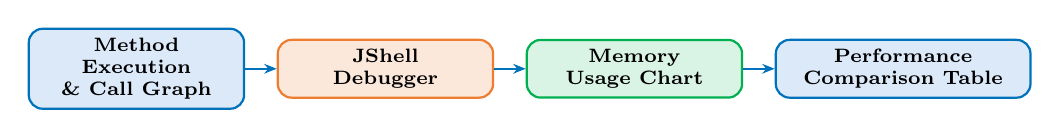
\begin{tikzpicture}[node distance=0.3cm and 0.25cm]
    \node[pbox,text width=2.5cm,font=\scriptsize\bfseries] (r1) {Method Execution\\\& Call Graph};
    \node[obox,text width=2.5cm,font=\scriptsize\bfseries,right=0.4cm of r1] (r2) {JShell\\Debugger};
    \node[gbox,text width=2.5cm,font=\scriptsize\bfseries,right=0.4cm of r2] (r3) {Memory\\Usage Chart};
    \node[pbox,text width=3.0cm,font=\scriptsize\bfseries,right=0.4cm of r3] (r4) {Performance\\Comparison Table};
    \draw[arr] (r1)--(r2); \draw[arr] (r2)--(r3); \draw[arr] (r3)--(r4);
  \end{tikzpicture}
  \end{center}
\end{frame}

% ── SLIDE 26 : RESULT 1 — METHOD EXECUTION + CALL GRAPH ─────
\begin{frame}{Results: Method Execution and Call Graph}
    \begin{figure}[htbp]
        \centering
        \includegraphics[
            width=1.0\textwidth,
            height=0.72\textheight,
            keepaspectratio
        ]{callgraph.png}
        
        \caption{Displays \textbf{execution time}, \textbf{call count}, and the \textbf{call graph}. \textcolor{DeepGreen}{\textbf{Insight:}} Highlights performance bottlenecks.}
        
        \label{fig:method_callgraph}
    \end{figure}
\end{frame}

% ── SLIDE 27 : RESULT 2 — JSHELL DEBUGGER ───────────────────
\begin{frame}{Results: JShell Debugger Output}
    \begin{figure}[htbp]
        \centering
        \includegraphics[
            width=1.0\textwidth,
            height=0.72\textheight,
            keepaspectratio
        ]{jshell.png}
        
        \caption{Interactive \textbf{JShell execution} for testing code snippets instantly. \textcolor{DeepGreen}{\textbf{Benefit:}} Faster debugging and quick validation.}
        
        \label{fig:jshell_output}
    \end{figure}
\end{frame}

% ── SLIDE 28 : RESULT 3 — MEMORY USAGE ──────────────────────
\begin{frame}{Results: Memory Usage Analysis}
    \begin{figure}[htbp]
        \centering
        \includegraphics[
            width=1.0\textwidth,
            height=0.75\textheight,
            keepaspectratio
        ]{memory.png}
        
        \caption{Displays \textbf{heap usage per class}. \textcolor{DeepGreen}{\textbf{Benefit:}} Helps detect memory leaks and optimize usage.}
        
        \label{fig:memory_analysis}
    \end{figure}
\end{frame}

% ── SLIDE 29 : PERFORMANCE COMPARISON TABLE ──────────────────
\begin{frame}{Results: Performance Comparison}
  \begin{block}{Impact of Using the Profiler}
    \small Testing shows \textbf{consistent improvements} in developer insight,
    debugging speed, and resource visibility.
  \end{block}
  \vspace{2pt}
  \footnotesize
  \renewcommand{\arraystretch}{1.3}
  \begin{table}
  \centering
  \begin{tabular}{|>{\columncolor{gradient1!20}}p{3.3cm}
                  |>{\columncolor{warning!20}}p{2.6cm}
                  |>{\columncolor{success!20}}p{2.6cm}
                  |>{\columncolor{info!20}}p{2.6cm}|}
    \hline
    \rowcolor{primary!80}
    \textbf{\color{white}Metric} &
    \textbf{\color{white}Without Profiler} &
    \textbf{\color{white}With Profiler} &
    \textbf{\color{white}Improvement} \\
    \hline
    Bottleneck Detection & Manual guesswork & Automated, precise & Instant accuracy \\
    \hline
    \rowcolor{SubtleGray}
    Memory Leak Identification & Hours of log analysis & Minutes via heap chart & $\sim$10$\times$ faster \\
    \hline
    Call Flow Understanding & Not available & Visual call graph & Full clarity \\
    \hline
    \rowcolor{SubtleGray}
    Debugging Complexity & High effort & Low (JShell) & Significantly reduced \\
    \hline
    Thread Activity Tracking & Invisible & Fully tracked & 100\% visibility \\
    \hline
    \rowcolor{SubtleGray}
    Method-level Timing & Not measurable & nanosecond precision & Granular insight \\
    \hline
  \end{tabular}
  \caption{\small Profiler benefit comparison for Java applications.}
  \end{table}
\end{frame}

% ══════════════════════════════════════════════════════════════
%  SECTION 8 — DISCUSSION
% ══════════════════════════════════════════════════════════════
\section{Discussion}

% ── SLIDE 30 : REAL-WORLD APPLICATIONS ──────────────────────
\begin{frame}{Discussion: Real-World Applications}
  \begin{columns}[T]
    
    % ── LEFT SIDE (FIRST APPEARS) ─────────────────────────────
    \column{0.48\textwidth}
      \begin{block}<1->{Performance Optimization}
        \small Identifies slow methods and optimizes code for \textbf{faster, more
        efficient} Java applications across all domains.
      \end{block}
      
      \vspace{4pt}
      
      \begin{block}<1->{Enterprise App Monitoring}
        \small Monitors large-scale Java systems to ensure \textbf{smooth operation}
        under heavy workloads and high concurrency.
      \end{block}
      
      \vspace{4pt}
      
      \begin{block}<1->{Web Application Tuning}
        \small Improves \textbf{response times} and user experience by pinpointing
        slow components in Spring or Jakarta EE apps.
      \end{block}
    
    
    % ── RIGHT SIDE (SECOND CLICK) ─────────────────────────────
    \column{0.48\textwidth}
      \begin{exampleblock}<2->{Education \& Learning}
        \small Powerful \textbf{teaching tool} for students to understand JVM
        internals, bytecode, and performance analysis hands-on.
      \end{exampleblock}
      
      \vspace{4pt}
      
      \begin{exampleblock}<2->{Testing \& Quality Assurance}
        \small Evaluates application behaviour under different \textbf{workloads during
        QA} to catch regressions before release.
      \end{exampleblock}
      
      \vspace{4pt}
      
      \begin{exampleblock}<2->{Resource Usage Analysis}
        \small Analyzes CPU usage and execution time for \textbf{better resource
        management} and cloud cost reduction.
      \end{exampleblock}

  \end{columns}
\end{frame}

% ── SLIDE 31 : CHALLENGES & SOLUTIONS ───────────────────────
\begin{frame}{Discussion: Challenges and Solutions}
  \begin{columns}[T]
    \column{0.48\textwidth}
    \vspace{-6pt}
      \begin{alertblock}{Challenges Faced}
        \begin{itemize}\small\itemsep3pt
          \item \textbf{Profiling Overhead} — instrumentation adds extra instructions,
                slightly slowing the target application.
          \item \textbf{Thread Safety} — concurrent method calls can corrupt shared data
                structures if not handled carefully.
          \item \textbf{JVM Compatibility} — JVMTI hooks differ across Java versions,
                breaking profiler on updates.
          \item \textbf{Large Call Graphs} — deeply recursive or highly connected programs
                produce graphs that are hard to visualize.
          \item \textbf{Data Volume} — high-frequency apps generate massive event streams
                that must be processed without lag.
        \end{itemize}
      \end{alertblock}
    \column{0.48\textwidth}
      \begin{exampleblock}{Solutions Applied}
        \begin{itemize}\small\itemsep4pt
          \item \textbf{ConcurrentHashMap} — thread-safe storage with no global locks.
          \item \textbf{Selective Instrumentation} — profile only critical packages,
                not third-party libraries.
          \item \textbf{Async Socket Transfer} — decouples data collection from UI
                rendering to prevent blocking.
          \item \textbf{Graph Pruning} — collapse small leaf nodes in call graph
                for readability.
          \item \textbf{Buffered Transmission} — batch events before sending to UI
                to reduce socket overhead.
        \end{itemize}
      \end{exampleblock}
  \end{columns}
\end{frame}

% ── SLIDE 32 : OPTIMIZATIONS & FUTURE ENHANCEMENTS ──────────
\begin{frame}{Discussion: Optimizations and Future Enhancements}
  \begin{columns}[T]
    \column{0.48\textwidth}
      \begin{block}{Current Optimizations}
        \begin{itemize}\small\itemsep3pt
          \item \textbf{ConcurrentHashMap} for zero-lock concurrent updates.
          \item \textbf{Buffered socket} transmission reduces UI lag.
          \item \textbf{Selective instrumentation} reduces overhead on non-critical code.
          \item \textbf{Graph pruning} keeps call graph readable even for large apps.
          \item \textbf{Nanosecond timestamps} ensure high-precision timing.
        \end{itemize}
      \end{block}
    \column{0.48\textwidth}
      \begin{block}{Future Enhancements}
        \begin{enumerate}\small\itemsep3pt
          \item \textbf{GC Tracking} — monitor garbage collection cycles and pauses.
          \item \textbf{Deadlock Detection} — detect and visualize thread deadlocks.
          \item \textbf{Real-time Dashboard} — charts with zoom, filter, and export.
          \item \textbf{Large-Scale Support} — handle high-load enterprise apps.
          \item \textbf{Sampling Mode} — statistical profiling for production use.
          \item \textbf{Automated Reports} — generate PDF/HTML performance summaries.
          \item \textbf{IDE Plugin} — integrate directly into IntelliJ or Eclipse.
        \end{enumerate}
      \end{block}
  \end{columns}
\end{frame}

% ══════════════════════════════════════════════════════════════
%  SECTION 9 — CONCLUSION
% ══════════════════════════════════════════════════════════════
\section{Conclusion}

% ── SLIDE 33 : CONCLUSION ───────────────────────────────────
\begin{frame}{Conclusion}
        \begin{enumerate}\small\itemsep4pt
          \item \textbf{Functionality Verified} — profiler correctly captures execution
                details across all tested programs.
          \item \textbf{Concepts Mastered} — deep understanding of Java agents,
                bytecode modification, and JVM internals.
          \item \textbf{Practical Skills} — learned to detect slow methods and analyze
                real-world execution data hands-on.
          \item \textbf{Seamless Integration} — Java agent, JVMTI, socket communication,
                and Swing UI work as one cohesive system.
          \item \textbf{Real-Time Monitoring} — continuous tracking makes debugging and
                optimization faster and more reliable.
          \item \textbf{Educational Value} — serves as a clear, hands-on guide to JVM
                profiling for students and developers.
        \end{enumerate}
  \begin{alertblock}{Final Thought}
    \centering
    \textbf{``Profiling is not just a tool — it is the lens through which
    developers see the true behaviour of software and transform complexity
    into clarity, performance, and reliability.''}
  \end{alertblock}
\end{frame}

% ══════════════════════════════════════════════════════════════
%  SECTION 10 — REFERENCES
% ══════════════════════════════════════════════════════════════
\section{References}
\begin{frame}[allowframebreaks]{References}
\small
\begin{thebibliography}{99}

\bibitem{burchell2023}
Burchell, T., \& Marr, S. (2023).
\textit{Don't Trust Your Profiler: An Empirical Study on the Precision and Accuracy of Java Profilers.}
MPLR.
\href{https://stefan-marr.de/downloads/mplr23-burchell-et-al-dont-trust-your-profiler.pdf}{[PDF Link]}

\bibitem{burchell2024}
Burchell, T., \& Marr, S. (2024).
\textit{Towards Realistic Results for Instrumentation-Based Profilers for JIT-Compiled Systems.}
MPLR.
\href{https://stefan-marr.de/downloads/mplr24-burchell-et-al-towards-realistic-results-for-instrumentation-based-profilers-for-jit-compiled-systems.pdf}{[PDF Link]}

\bibitem{ase2024}
Automated Software Engineering Research Team. (2024).
\textit{Comparing CPU and Memory Profiler Results Across Multiple Java Versions.}
Springer.
\href{https://link.springer.com/article/10.1007/s10515-024-00423-2}{[Link]}

\bibitem{pj2023}
Programming Journal Research Team. (2023).
\textit{Profiling and Optimizing Java Streams.}
Programming Journal.
\href{https://programming-journal.org/2023/7/10/}{[Link]}

\bibitem{softx2024}
SoftwareX Research Team. (2024).
\textit{JVM Optimization: An Empirical Analysis of JVM Configurations for Enhanced Web Application Performance.}
SoftwareX / ScienceDirect.
\href{https://www.sciencedirect.com/science/article/pii/S2352711024003030}{[Link]}

\bibitem{acm2022}
ACM Research Publication. (2022).
\textit{Optimal Heap Limits for Reducing Browser Memory Use.}
ACM Digital Library.
\href{https://dl.acm.org/doi/epdf/10.1145/3563323}{[Link]}

\end{thebibliography}
\end{frame}

% ── SLIDE 35 : THANK YOU ─────────────────────────────────────
\begin{frame}[plain]
  \begin{tikzpicture}[remember picture,overlay]
    \fill[PrimaryBlue!92]
      (current page.south west) rectangle (current page.north east);
    \fill[AccentOrange]
      ([yshift=-0.5cm]current page.north west)
      rectangle ([yshift=-0.85cm]current page.north east);
    \fill[AccentOrange]
      ([yshift=0.5cm]current page.south west)
      rectangle ([yshift=0.85cm]current page.south east);
  \end{tikzpicture}
  \vspace{1.4cm}
  \begin{center}
    {\Huge\bfseries\color{white} Thank You!}\\[12pt]
    {\large\color{white!90} Questions \& Feedback Welcome}\\[18pt]
    \begin{tikzpicture}
      \node[draw=white,rounded corners=6pt,fill=white!15,
            text width=8cm,minimum height=1.0cm,text centered,
            font=\small\color{white}] {%
        M N Risheendra (241U1R1080) \quad
        K.\ Jwalin (241U1R1088) \quad
        Ankit Lama (241U1R1089)};
    \end{tikzpicture}
    \\[8pt]
    {\small\color{white!75}
      Dept.\ of CSE --- Aurora Higher Education and Research Academy, Hyderabad}\\[4pt]
    {\small\color{white!75}
      Guide: Dr.\ Vemula Aruna, Associate Professor}
  \end{center}
\end{frame}

% \begin{frame}
%     \centering
%     \Huge \textcolor{primary}{\textbf{Thank You!}} \\
%     \vspace{1cm}
%     \large \textbf{Questions?}
% \end{frame}

\end{document}\end{document}